
%(BEGIN_QUESTION)
% Copyright 2010, Tony R. Kuphaldt, released under the Creative Commons Attribution License (v 1.0)
% This means you may do almost anything with this work of mine, so long as you give me proper credit

Suppose you are asked to check the calibration of a control valve before wires have been pulled to that location from a controller output.  Process fluid is flowing through the pipe, bypassing the control valve until such time it is ready to be placed into service.  The only piece of calibrated test equipment you have with you, though, is a 4-20 mA loop calibrator with an inoperative ``Source'' mode.  The calibrator can measure and simulate 4-20 mA just fine, but it cannot {\it source} 4-20 mA.

$$\includegraphics[width=15.5cm]{i03617x01.eps}$$

Show how you could still (creatively) use the loop calibrator to stroke the valve despite its lacking functionality -- feel free to add any other electronic component(s) as necessary to make it work.  Then, calculate the necessary current to send to the valve to make it open to 75\%, assuming a split-range calibration of 12 mA (closed) to 20 mA (open).

\vskip 10pt

Also, determine the necessary hand-valve settings (fully shut, fully open, or partially open) in order to bypass flow around the control valve but maintain operator (manual) control over the flow rate, and determine which (if any) of these manual valves must be {\it locked} and {\it tagged} for safety while the control valve remains unfit for service.

\vfil

\underbar{file i03617}
\eject
%(END_QUESTION)





%(BEGIN_ANSWER)

This is a graded question -- no answers or hints given!

%(END_ANSWER)





%(BEGIN_NOTES)

The I/P is an electrical load, and so we need a {\it source} to drive 4-20 mA to it.  Since the calibrator's source mode is not working, we must get creative with how we use it. 

One solution is to set the loop calibrator to {\it simulate} 18 mA of current, connected as an electrical {\it load} in series with a DC voltage source and the I/P converter:

$$\includegraphics[width=15.5cm]{i03617x02.eps}$$

Another solution would be to set the loop calibrator to the {\it measure} (``read'') mode, then use a variable current source in series to drive current to the I/P, using the loop calibrator simply as an ammeter.

\vskip 10pt

Both block valves must be fully shut and locked, while the bypass valve remains partially open (and unlocked so that the operators may still move its position as needed).

%INDEX% Electronics review: 4-20 mA loop calibrator (test equipment)

%(END_NOTES)


